\chapter{Evaluation}
\label{ch_evaluation}

This chapter explains the basics of working with PRISM model checker,
then describes how are the algorithms implemented as a part of PRISM and
how do they compare to other methods on standard models.
(TODO: In the last section we make some observations relating the model
structure with the performance of the methods).

\section{PRISM, Probabilistic Model Checker}

PRISM \parencite{prism}
({\em probabilistic model checker}) is a program/framework
for formal modelling and analysis of probabilistic systems.
We show how to use PRISM to describe MDPs, their properties,
and how to check them.

\subsection*{Describing MDPs with the PRISM language}
PRISM has a language for description of Markov decision processes
based on the formalism of Alur and Henzinger \parencite{ReactiveModules}.
A brief example is given below for the readers who wish to try our
algorithms on small models which they can describe and solve by hand.
The the definitive guide to the language is available online on the
PRISM homepage \parencite{prism_lang}.

The PRISM language describes {\em modules} (interacting actors),
their states (using variables) and transitions between the states.
An example single PRISM language line is below. The line translates as:
if condition \verb|guard| is satisfied the actor can choose action \verb|act|
and
with probability \verb|prob_1| update \verb|update_1| will happen,
with probability \verb|prob_2| update \verb|update_2| will happen,
and so on.

\begin{verbatim}
[act] guard -> prob_1 : update_1 + prob_2 : update_2 + ...
\end{verbatim}

An example module is described below and is equivalent to the MDP
depicted in \autoref{moduleM}.

\smallskip
\begin{verbatim}
mdp // Tell PRISM this file describes an MDP
module M
    s : [0 .. 3] init 0;
    [a] s=0 -> (s'=0);
    [b] s=0 -> 0.9:(s'=1) + 0.1:(s'=0);
    [c] s=1 -> 0.9:(s'=2) + 0.1:(s'=1);
    [d] s=2 -> (s'=2);
endmodule
\end{verbatim}
\smallskip

\begin{figure}
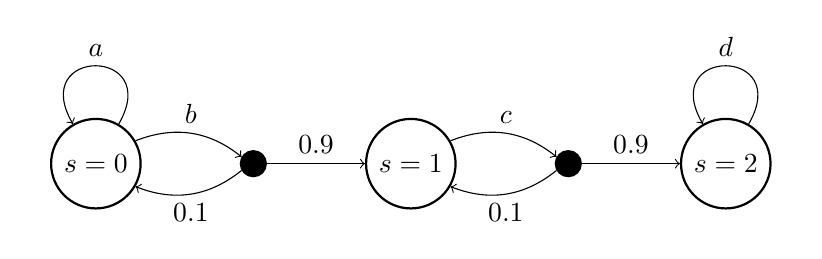
\begin{tikzpicture}
    \tikzstyle{state}=[thick,draw=black,circle]
    \tikzstyle{transition}=[draw,shape=circle,fill=black]
    \tikzstyle{loop}=[looseness=5, in=120, out=60]

    \node[state] at (0,0) (s0) {$s = 0$};
    \node[transition] at (2,0) (s0b) {};
    \node[state] at (4,0) (s1) {$s = 1$};
    \node[transition] at (6,0) (s1b) {};
    \node[state] at (8,0) (s2) {$s = 2$};

    \draw (s0) edge [loop,->] node [above] {$a$} (s0);

    \draw (s0) edge [bend left, ->] node [midway, above] {$b$} (s0b);
    \draw[->] (s0b) -- (s1) node [midway, above] {0.9};
    \draw (s0b) edge [bend left, ->] node [midway, below] {0.1} (s0);

    \draw (s1) edge [bend left, ->] node [midway, above] {$c$} (s1b);
    \draw[->] (s1b) -- (s2) node [midway, above] {0.9};
    \draw (s1b) edge [bend left, ->] node [midway, below] {0.1} (s1);

    \draw (s2) edge [loop,->] node [above] {$d$} (s2);
\end{tikzpicture}
\caption{Module M}
\label{moduleM}
\end{figure}

A property we might be interested in is the maximum probability of
eventually reaching state \verb|s=2|.  TODO: Describe the logic.
TODO: Warn that only support Pmax and we don't support timed properties (e.g. $F <=
x$ is not supported).

\subsection*{Running PRISM}

We have a model description and a property but before we analyze it
PRISM has to be installed.
There is a modified version of PRISM distributed with this thesis. It
can be built by issuing the \verb|make| command inside the
\verb|prism| directory. Java is a required prerequisite.
Once built the PRISM binary is available at \verb|prism/bin/prism|.

Now use PRISM to analyze the model -- its name is passed as the first
argument and \verb|-pf| specifies the property we want to check.
The \verb|-ex| flag will be described later.
Running the command below
confirms our expectations: the maximum probability of eventually
reaching state \verb|s=2| is 1.

\medskip
\begin{verbatim}
./prism modelM.nm -pf 'Pmax=? [F s=2]' -ex
\end{verbatim}
\medskip

The following tells PRISM to use MCTS-BRTDP where the next state in
BRTDP is chosen to be the one with highest upper bound.

\medskip
\begin{verbatim}
./prism modelM.nm -pf 'Pmax=? [F s=2]' -heuristic_verbose \
 -heuristic MCTS_BRTDP -next_state HIGH_PROB
\end{verbatim}
\medskip

The UCB exploration constant can be chosen with the
\verb|-ucb1constant v|. If not provided the value is set to
$1/\sqrt{2}$.

The method can be chosen out of the following: \verb|MCTS_BRTDP|,
\verb|MCTS| (TODO: Rename to BMCTS), \verb|BRTDP|, \verb|BRTDP_UCB|,
or empty for value  iteration.
The next state heuristics are
\verb|HIGH_PROB|, \verb|MAX_DIFF|.
The variation of BRTDP using UCB to select the next action is chosen by
adding switch \verb|-next_action 2|.

\subsection*{Data structures}
The \verb|-ex| switch used in the value iteration example above tells
PRISM to use the explicit computation engine.
The explicit computation engine explores the MDP and stores it in
a sparse matrix before the value iteration algorithm is run.

PRISM offers three symbolic computation engines based on binary decision
diagrams, namely MTBDD (multi-terminal BDD, \verb|-mtbdd| switch),
sparse TODO.

All the heuristic methods use a data structure implemented in
\verb|prism/src/heuristic/CachedModelGenerator.java|.
With this {\em model generator} data structure PRISM will not build the
whole MDP from its description unless asked to.
Asking the model generator to reveal parts of the model results in the
construction of an {\em explicit model} which is cached in the memory.
Such construction is computationally expensive and often unnecessary
which is when the heuristic methods perform so well.

\section{Implementation}

We describe how the pseudocode described in \autoref{ch_mcts} maps to
the implementation in PRISM. The implementation can be found in
\verb|prism/src/heuristics|.

To represent the MCTS tree we use classes \verb|MCTree.java| and
\linebreak
\verb|MCNode.java|. The tree class has an important method \verb|unfold|
which asks the model generator to add the next states of a given state
to the explicit model and adds them to the tree.

The next state heuristics are implemented in a straightforward way
inside directory \verb|nextstate|. The UCB heuristic is implemented in
directory \verb|treeheuristic|.

MCTS-BRTDP is implemented in \verb|search/MctsBrtdp.java|. The entry
point is method \verb|computeProb|, subsequently
\verb|monteCarloTreeSearch| is invoked until the stopping condition
is reached (see method \verb|isDone|). Method
\verb|monteCarloTreeSearch| first selects and expands a tree state,
then uses \verb|exploreAndUpdate| implemented in BRTDP
(\verb|search/HeuristicBrtdp.java|) as the default policy and propagates
the values using updates to the root.

TODO: Describe treeSelectAndExpand?

BMCTS is implemented by modifying MCTS-BRTDP. The modification is turned
on when the flag \verb|next_action 5| is added to a command using
MCTS-BRTDP. This change makes the BRTDP implementation chose next action
uniformly at random instead of the BRTDP-way by upper bound.

\section{Models}

Experimental evaluation was done on standard models
distributed with PRISM. Most of the MDPs described by these models are
concerned with network configuration where randomness plays important
role in achieving a common goal. We provide a brief description of each
model and refer the reader to thorough description on PRISM's website.
http://www.prismmodelchecker.org/casestudies/

The description of the models in the PRISM language can be found inside
\verb|tests/reachability/models| in the source codes attached to this
thesis.

TODO: Do only two or three which we will discuss later.

\subsection*{Zero-configuration networking}

{\em Zeroconf} model corresponds to a set of computers establishing a
network without a given leader. Such leader could be a human setting
static IP addresses or a DHCP server which would need to be configured
up front -- in both cases there is extra work required.

The zero-configuration networking protocol describes how should the
computers proceed. Upon connecting to the network a computer picks an IP
address at random and broadcasts its choice via an ARP packet called
{\em probe} repeated $K$ times ($K=4$ by the standard) with two second
delay. If another computer responds to one these
ARP packets the original sender will then pick another IP address and
repeat the process. If it does not receive a response it then broadcasts
twice an ARP packet asserting this computer's use of the chosen IP
address.

TODO: defering and stuff, just one paragraph

To summarize, the model describes $N$ computers establishing a network,
each sending $K$ probes to inform the others of its choices.

\subsection*{IEEE 1394 FireWire}

FireWire is an interface standard for serial bus

\subsection*{Wireless LAN}

\subsection*{Randomised Consensus Shared Coin Protocol}

\subsection*{Asynchronous Leader Election Protocol}

\subsection*{mer}

\section{Experimental Comparison}

On the following pages we present the results of our measurements. TODO:
describe the machine and JVM configuration. TODO: set up an example
runbenchmarks script so that anyone can verify our results right away.

The tables show that MCTS based methods are clear winners on the
zeroconf model but also clear losers on the

In the following section we try to derive some reasons for this results
and generalize.

\begin{landscape}
\begin{tabular}{ l  | c | c  }
zeroconf   &    BRTDP\_UCB=None    &     VI\_UCB=None      \\
N=4;K=4    &                0.162 &               15.321 \\
\end{tabular}
\end{landscape}

\section{Behaviour on Small Models}

Describe how do MCTS based methods solve few small models like bin tree

\section{Model Structure and MCTS Performance}

We discuss what are the possible reasons MCTS performs well on some
models and worse on others. (See e.g. On Adversarial Search Spaces and
Sampling-Based Planning for a similar comparison between MCTS on Chess
and Go).

From the Chess and Go comparison it would seem that MCTS based methods would
not perform well in verification as there are usually many dead ends.
However by tuning the parameters and trying variants of the algorithms
we have achieved better results on several models than other known methods.

TODO :-/

can we extrapolate where will each method do well from small instances of the models?
